%!TEX root = ../thesis.tex
% ******************************* Thesis Appendix E ****************************
\cleardoublepage
\chapter{R\'{e}sum\'{e} \'{e}tendu de la thèse}
\label{apx:E}
%*******************************************************************************
\selectlanguage{french}
%============================================================%
%============================================================%
\section*{Introduction}
%============================================================%
%============================================================%

%============================================================%
\subsection*{Contexte industriel}
%============================================================%

%{\color{red} citer qq ref pour asseoir ce que tu dis sur le contexte}

L'enjeu actuel de la transition \'{e}nerg\'{e}tique implique, entre autres, de r\'{e}duire la part des \'{e}nergies fossiles au sein du mix \'{e}lectrique mondial. 
Dans ce contexte, l'\'{e}nergie \'{e}olienne en mer pr\'{e}sente plusieurs avantages \citep{eolien_en_mer_2022}. 
L'\'{e}olien en mer b\'{e}n\'{e}ficie notamment de vents plus constants que l'\'{e}olien terrestre, notamment dû à l'absence de relief, et offre la possibilit\'{e} d'installer des \'{e}oliennes plus grandes donc plus puissantes. 
Depuis l'installation de la première ferme \'{e}olienne en mer à Vindeby, au Danemark, en 1991, l'industrie a connu une croissance rapide, avec une capacit\'{e} totale de 56 GW exploit\'{e}e dans le monde en 2021. 
Au fil du temps, la technologie \'{e}olienne en mer s'est am\'{e}lior\'{e}e, aboutissant à des succès importants tels que la signature de projets non subventionn\'{e}s en Europe (en anglais \textit{zero-subsidy bids}), pour lesquels l'\'{e}lectricit\'{e} produite est directement vendue sur le march\'{e} de gros \citep{eolien_en_mer_2022}.

Cependant, malgr\'{e} les progrès techniques ind\'{e}niables, des limites industrielles \'{e}mergent vis-à-vis de ces parcs \'{e}oliens en mer, posant ainsi de nombreux d\'{e}fis scientifiques. 
Pour atteindre les ambitieux objectifs de d\'{e}veloppement au niveau national et r\'{e}gional, la filière de l'\'{e}olien en mer fait face à plusieurs problèmes li\'{e}s à l'augmentation de la taille des turbines.
Ce changement d'\'{e}chelle cr\'{e}e notamment des tensions li\'{e}es à la logistique portuaire, aux besoins en ressources primaires et à la gestion durable du d\'{e}mantèlement futur. 
Ce secteur pr\'{e}sente plusieurs d\'{e}fis techniques et scientifiques, qui requièrent l'utilisation conjointe de donn\'{e}es mesur\'{e}es et de simulations num\'{e}riques d'\'{e}oliennes dans leur environnement. 
La recherche appliqu\'{e}e à l'\'{e}olien en mer fait intervenir plusieurs disciplines qui \'{e}tudient notamment des sujets tels que la conception d'\'{e}oliennes flottantes, l'am\'{e}lioration de l'estimation des ressources \'{e}oliennes, l'optimisation des op\'{e}rations de maintenance et l'augmentation de la dur\'{e}e de vie utile des parcs. 
De manière g\'{e}n\'{e}rale, plusieurs d\'{e}cisions sont prises durant la vie d'une \'{e}olienne par son concepteur, installateur et exploitant, tout en ayant une connaissance partielle de certains ph\'{e}nomènes physiques. 
Par cons\'{e}quent, mod\'{e}liser et maîtriser les diverses sources d'incertitudes associ\'{e}es à l'\'{e}olien en mer s'avère être un \'{e}l\'{e}ment d\'{e}terminant dans une industrie hautement concurrentielle.

Dans l'ensemble, l'industrie de l'\'{e}olien en mer a besoin de m\'{e}thodes de traitement des incertitudes pour maîtriser les marges de sûret\'{e} et la gestion des actifs industriels (à la maille des composants, de l'\'{e}olienne et du parc dans son ensemble, \citealp{OWT_review_2016}). 
Pour un d\'{e}veloppeur de projets \'{e}oliens, l'attention est d'abord port\'{e}e sur l'am\'{e}lioration du potentiel \'{e}olien des sites candidats en combinant diff\'{e}rentes sources d'information et en mod\'{e}lisant la distribution multivari\'{e}e des conditions environnementales au sein d'un parc \'{e}olien. 
Dans le cas de projets en \'{e}olien flottant, l'objectif est d'int\'{e}grer un aspect probabiliste dès la phase de conception (par exemple, du flotteur) afin de d\'{e}finir des solutions plus sûres, plus robustes et plus rentables. 
Pour un propri\'{e}taire d'un parc \'{e}olien, la gestion de la fin de vie est une autre probl\'{e}matique importante. 
Un propri\'{e}taire de parc \'{e}olien en fin de vie à le choix entre trois options : prolonger la dur\'{e}e de vie des actifs en exploitation, remplacer les \'{e}oliennes actuelles par des modèles plus r\'{e}cents, ou d\'{e}manteler et vendre le parc \'{e}olien. 
Les deux premières solutions n\'{e}cessitent d'\'{e}valuer la fiabilit\'{e} de la structure et sa dur\'{e}e de vie r\'{e}siduelle. Ces \'{e}valuations quantitatives sont examin\'{e}es par des organismes de certification et des assureurs pour d\'{e}livrer des permis d'exploitation. 
Pour fournir des \'{e}valuations rigoureuses des risques, la m\'{e}thodologie g\'{e}n\'{e}rique de \textit{traitement des incertitudes} est une d\'{e}marche qui fait consensus dans les secteurs industriels confront\'{e}s à ce genre de probl\'{e}matique \citep{rocquigny_2008,blanchard_2023}.


%============================================================%
\subsection*{M\'{e}thodologie g\'{e}n\'{e}rique de traitement des incertitudes dans les outils de calcul scientifiques}
%============================================================%

La simulation num\'{e}rique est une discipline qui a \'{e}merg\'{e} avec l'avènement de l'informatique. 
Cette pratique produit des outils de calcul scientifique (OCS) qui permettent de simuler le comportement de système complexes compte tenu de conditions initiales d\'{e}finies par l'analyste. 
Les OCS sont vite devenus indispensables pour l'analyse, la conception, et la certification de systèmes complexes dans les cas o\`u des exp\'{e}riences ou des mesures physiques sont coûteuses à obtenir, voire impossibles à r\'{e}aliser. 
Cependant, ces modèles num\'{e}riques s'intègrent dans une d\'{e}marche d\'{e}terministe : le r\'{e}sultat d'une simulation est associ\'{e} à un vecteur de paramètres fix\'{e} en entr\'{e}e. 
La question de la gestion des incertitudes associ\'{e}es aux entr\'{e}es se pose rapidement lors de l'utilisation des OCS. 

Le traitement des incertitudes vise à mod\'{e}liser et à traiter les incertitudes autour d'un modèle num\'{e}rique. 
Pour ce faire, une m\'{e}thodologie g\'{e}n\'{e}rique a \'{e}t\'{e} propos\'{e}e pour quantifier et analyser les incertitudes entre les variables d'entr\'{e}e et de sortie d'un OCS \citep{rocquigny_2008,blanchard_2023}. 
Une pr\'{e}sentation des outils math\'{e}matiques utilis\'{e}s dans ce domaine est propos\'{e}e par \citet{sullivan_2015}.
Cette approche apporte une meilleure compr\'{e}hension d'un système, ce qui contribue à une prise de d\'{e}cision plus robuste.   


La Figure \ref{fig:UQ_methodo_FR} illustre les \'{e}tapes g\'{e}n\'{e}riques de la m\'{e}thodologie de quantification des incertitudes, qui sont brièvement d\'{e}crites ci-après :
\begin{itemize}
    \item[\textbullet] \textbf{\'Etape A -- Sp\'{e}cification du problème.} 
    Cette \'{e}tape consiste à d\'{e}terminer le système \'{e}tudi\'{e} et construire un modèle num\'{e}rique capable de simuler (pr\'{e}cis\'{e}ment) son comportement. 
    La sp\'{e}cification du problème implique \'{e}galement de d\'{e}finir l'ensemble des paramètres inh\'{e}rents au modèle num\'{e}rique. 
    Ces paramètres comprennent aussi bien les variables d'entr\'{e}e que les variables de sortie g\'{e}n\'{e}r\'{e}es par la simulation. 
    Dans ce document, le modèle num\'{e}rique est consid\'{e}r\'{e} comme une boîte-noire, par opposition à des approches qui s'intègrent à l'int\'{e}rieur des sch\'{e}mas de r\'{e}solution num\'{e}rique des \'{e}quations de comportement du système (approches dites intrusives \citealp{lemaitre_2010}). 
    En g\'{e}n\'{e}ral, ces modèles num\'{e}riques sont au pr\'{e}alable calibr\'{e}s par rapport à des donn\'{e}es mesur\'{e}es et suivent un processus de validation et de v\'{e}rification pour r\'{e}duire les erreurs de mod\'{e}lisation \citep{oberkampf_2010_VVUQ,damblin_2015,carmassi_2018}.
    \item[\textbullet] \textbf{\'Etape B -- Mod\'{e}lisation et quantification des incertitudes.} 
    L'objectif de la deuxième \'{e}tape est d'identifier et mod\'{e}liser toutes les sources d'incertitude associ\'{e}es aux variables d'entr\'{e}e. 
    Dans la plupart des cas, cette mod\'{e}lisation est effectu\'{e}e dans un cadre probabiliste.
    \item[\textbullet] \textbf{\'Etape C -- Propagation des incertitudes.} 
    Lors de cette \'{e}tape, les entr\'{e}es incertaines sont propag\'{e}es au travers du modèle de simulation num\'{e}rique. 
    Dès lors, la sortie du modèle num\'{e}rique (habituellement de type scalaire) devient \'{e}galement incertaine. 
    L'objectif est alors d'estimer une quantit\'{e} d'int\'{e}rêt, c'est-à-dire une statistique sur la variable al\'{e}atoire de sortie \'{e}tudi\'{e}e. 
    La m\'{e}thode de propagation de l'incertitude peut diff\'{e}rer en fonction de la quantit\'{e} d'int\'{e}rêt vis\'{e}e (par exemple, la tendance centrale, un quantile, une probabilit\'{e} d'\'{e}v\'{e}nement rare). 
    \item[\textbullet] \textbf{\'Etape C' -- Analyse de sensibilit\'{e}.} 
    En compl\'{e}ment de la propagation d'incertitudes, une analyse de sensibilit\'{e} peut être r\'{e}alis\'{e}e afin d'\'{e}tudier le rôle attribu\'{e} à chaque entr\'{e}e incertaine dans la variabilit\'{e} de la sortie d'int\'{e}rêt.
    \item[\textbullet] \textbf{M\'{e}tamod\'{e}lisation.} 
    Compte tenu du coût de calcul \'{e}lev\'{e} que repr\'{e}sentent certaines simulations, des approches statistiques visent à \'{e}muler ces simulateurs coûteux partir d'un nombre limit\'{e} de simulations. 
    La quantification de l'incertitude peut alors être r\'{e}alis\'{e}e avec le m\'{e}tamodèle (ou modèle de substitution) pour un moindre coût de calcul. 
    Cette \'{e}tape optionnelle d'apprentissage statistique ne fait pas à proprement dit partie du traitement des incertitudes mais elle s'avère souvent essentielle pour permettre sa mise en \oe uvre pratique. 
\end{itemize}

\begin{figure}[!h]
    \centering
    %\begin{figure}[h]
%    \centering
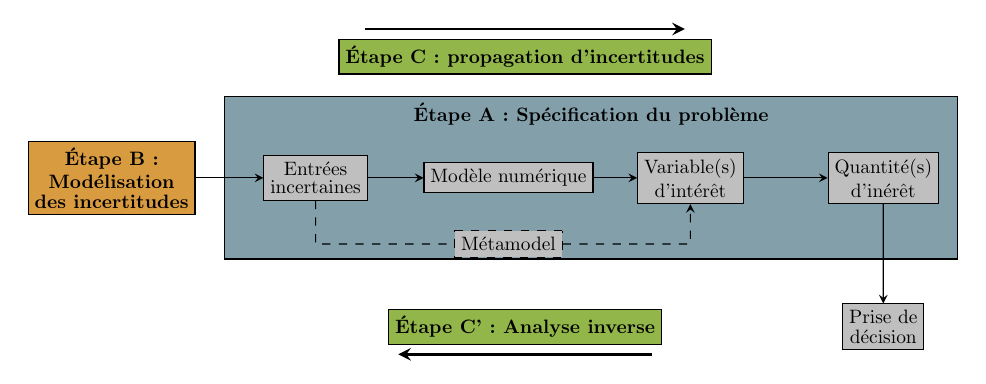
\begin{tikzpicture}[scale=0.7, every node/.style={transform shape}]
    \node[rectangle,draw,fill=YellowOrange!70!gray] (a) at (-9,0) {\shortstack{\textbf{\'Etape B :} \\ \textbf{Mod\'{e}lisation} \\ \textbf{des incertitudes}}};
\node[rectangle,draw,fill=YellowGreen!70!gray] (f) at (-1.5,2.2) {
\textbf{\'Etape C : propagation d'incertitudes}};
\node[rectangle,draw,fill=YellowGreen!70!gray] (g) at (-1.5,-2.7) {\shortstack{
\textbf{\'Etape C' : Analyse inverse}}};
\node[rectangle,draw,minimum width=13.3cm,fill=SkyBlue!40!gray] (h) at (-0.3,0) {\shortstack{\textbf{\'Etape A : Sp\'{e}cification du problème} \\ \phantom{a} \\ \phantom{a} \\ \phantom{a} \\ \phantom{a} \\ \phantom{a} \\ \phantom{a} \\ \phantom{a} \\ \phantom{a} \\ \phantom{a} }};
\node[rectangle,draw,fill=lightgray] (b) at (-5.3,0) {\shortstack{
Entr\'{e}es\\ incertaines}};
\node[rectangle,draw,fill=lightgray] (c) at (-1.8,0) {\shortstack{
    Modèle num\'{e}rique}};
\node[rectangle,draw,fill=lightgray] (d) at (1.5,0) {\shortstack{
Variable(s) \\ d'int\'{e}rêt}};
\node[rectangle,draw,fill=lightgray] (e) at (5,0) {\shortstack{
Quantit\'{e}(s) \\ d'in\'{e}rêt}};
\node[rectangle,draw,fill=lightgray, dashed] (i) at (-1.8,-1.2) {M\'{e}tamodel};
\node[rectangle,draw,fill=lightgray] (j) at (5,-2.7) {\shortstack{Prise de \\ d\'{e}cision}};
\draw[-stealth, black, line width=1pt] (-4.4,2.7) -- (1.4,2.7);
\draw[-stealth, black, line width=1pt] (0.8,-3.2) -- (-3.8,-3.2);
\draw[-stealth, black] (a) -- (b);
\draw[-stealth, black] (b) -- (c);
\draw[-stealth, black] (c) -- (d);
\draw[-stealth, black] (d) -- (e);
\draw[-stealth, black, dashed] (b) -- (-5.3,-1.2) -- (i) -- (1.5,-1.2) -- (d);
 \draw[-stealth, black] (e) -- (j);

\end{tikzpicture}
%    \caption{General uncertainty quantification and propagation framework}
%    \label{Fig:UQ}
%\end{figure}
    \caption{Sch\'{e}ma g\'{e}n\'{e}rique de la quantification des incertitudes (\citealp{rocquigny_2008}, adapt\'{e} par \citealp{ajenjo_2023}).}
    \label{fig:UQ_methodo_FR}
\end{figure}


%============================================================%
\subsection*{Verrous scientifiques et objectifs de la thèse}
%============================================================%

La maîtrise des risques et des incertitudes dans l'\'{e}olien est un enjeu majeur pour le groupe EDF en tant qu'exploitant. 
Cette thèse vise à adapter et appliquer, sur un cas d'usage issu de l'\'{e}olien en mer, une d\'{e}marche globale de traitement des incertitudes. 
Ainsi, ce cas d'usage soulève des verrous scientifiques associ\'{e}s à ses particularit\'{e}s qui peuvent être d\'{e}crites comme suit :
\begin{itemize}
    \item[\textbullet] 
    Le code de simulation num\'{e}rique autour duquel les travaux sont r\'{e}alis\'{e}s est constitu\'{e} d'une chaîne de codes de calcul, ex\'{e}cut\'{e}s en s\'{e}rie. 
    Cette chaîne s'articule en trois \'{e}tapes : d'abord une g\'{e}n\'{e}ration temporelle et stochastique d'un champ de vitesse de vent et de houle, puis la simulation du comportement hydro-a\'{e}ro-servo-\'{e}lastique de l'\'{e}olienne et enfin une phase d'agr\'{e}gation des r\'{e}sultats temporels pour obtenir des quantit\'{e}s d'int\'{e}rêt scalaires;
    \item[\textbullet] 
    La complexit\'{e} de cet outil de calcul scientifique ainsi que le coût de calcul unitaire \'{e}lev\'{e} (de l'ordre de 20 minutes par simulation) n\'{e}cessite l'utilisation de m\'{e}thodes d'\'{e}chantillonage performantes, ainsi que des systèmes de calcul haute performance. 
    En plus de la complexit\'{e} li\'{e}e au modèle num\'{e}rique, la mod\'{e}lisation des incertitudes en entr\'{e}e pr\'{e}sente, elle aussi, des difficult\'{e}s. 
    En effet, la loi conjointe des conditions environnementales li\'{e}es à un site comporte une structure de d\'{e}pendance complexe à capturer et à mod\'{e}liser. 
    L'\'{e}tape d'inf\'{e}rence vis-à-vis des grandes quantit\'{e}s de donn\'{e}es mesur\'{e}es est d'autant plus importante que sa qualit\'{e} impacte directement les conclusions de la propagation d'incertitudes.
\end{itemize}

Afin d'appliquer le sch\'{e}ma global de traitement des incertitudes au cas \'{e}olien, cette thèse vise à r\'{e}pondre aux probl\'{e}matiques suivantes :
\begin{itemize}
    \item[\textbf{Q1.}] \textit{
    Comment pr\'{e}cis\'{e}ment mod\'{e}liser la structure de d\'{e}pendance complexe associ\'{e}e aux lois conjointes de conditions environnementales ?
    } (\ding{238} \'Etape B)
    \item[\textbf{Q2.}] \textit{
    Comment r\'{e}aliser une propagation d'incertitudes au travers d'une chaîne de simulation num\'{e}rique coûteuse, uniquement bas\'{e}e sur une description empirique (donn\'{e}es mesur\'{e}es) des incertitudes en entr\'{e}e ?
    } (\ding{238} \'Etape C)
    \item[\textbf{Q3.}] \textit{
    Comment estimer des probabilit\'{e}s d'\'{e}v\'{e}nements rares associ\'{e}es à la ruine de structures \'{e}oliennes en mer ?
    } (\ding{238} \'Etape C)
    \item[\textbf{Q4.}] \textit{
    Comment \'{e}valuer et interpr\'{e}ter la sensibilit\'{e} des entr\'{e}es incertaines vis-à-vis des quantit\'{e}s d'int\'{e}rêt li\'{e}es à la fiabilit\'{e} des structures (analyse de sensibilit\'{e} fiabiliste) ?
    } (\ding{238} \'Etape C')
\end{itemize}
Les sections suivantes r\'{e}sument les travaux de thèse, tout en respectant la structure du manuscrit. 



%============================================================%
%============================================================%
\section*{R\'{e}sum\'{e}s des chapitres relatifs à l'\'{e}tat de l'art des m\'{e}thodes et outils mis en \oe{}uvre dans la thèse}
%============================================================%
%============================================================%


Les deux premiers chapitres relateront l'\'{e}tat de l'art dans le domaine du traitement des incertitudes et de la mod\'{e}lisation num\'{e}rique des systèmes \'{e}oliens. 

%------------------------------------------------------------%
\subsection*{Chapitre 1 -- Traitement des incertitudes en simulation num\'{e}rique}
%------------------------------------------------------------%
Ce chapitre vise à pr\'{e}senter un \'{e}tat de l'art concis des diff\'{e}rentes th\'{e}matiques en quantification des incertitudes \citep{sullivan_2015}. 
Après un rappel de quelques pr\'{e}requis math\'{e}matiques, l'\'{e}tape de sp\'{e}cification du modèle num\'{e}rique (consid\'{e}r\'{e} comme \'{e}tant une boîte-noire), ainsi que les variables d'entr\'{e}e et de sortie est d\'{e}taill\'{e}e. 
Les diff\'{e}rents types et sources d'incertitudes sont ensuite pr\'{e}sent\'{e}s, ainsi que leur mod\'{e}lisation dans un cadre probabiliste. 
La propagation des incertitudes d\'{e}pend de la nature des quantit\'{e}s d'int\'{e}rêt estim\'{e}es, ainsi, une section aborde les m\'{e}thodes de propagation pour l'\'{e}tude en tendance centrale et une autre s'int\'{e}resse aux problèmes d'estimation de probabilit\'{e}s d'\'{e}v\'{e}nements rares (statistiques li\'{e}es aux queues de distributions). 
La section d\'{e}di\'{e}e à la tendance centrale pr\'{e}sente des m\'{e}thodes d'int\'{e}gration num\'{e}rique, d'\'{e}chantillonnage et de planification d'exp\'{e}riences \citep{fang_liu_2018}. 
Celle consacr\'{e}e aux probabilit\'{e}s d'\'{e}v\'{e}nements rares pr\'{e}sente des m\'{e}thodes classiques issues du domaine de la fiabilit\'{e} des structures \citep{lemaire_2009,MorioBalesdent2015}.

Ce chapitre aborde \'{e}galement les principales m\'{e}thodes d'analyse de sensibilit\'{e} globale \citep{daveiga_iooss_2021}. 
Ce domaine divise ses m\'{e}thodes en deux grandes classes : les m\'{e}thodes de criblage et les mesures d'importance. 
D'une part, les techniques de criblage, g\'{e}n\'{e}ralement mises en \oe{}uvre dans les problèmes de grande dimension, visent à identifier les variables n'ayant qu'un faible impact sur la variabilit\'{e} de la sortie d'int\'{e}rêt. 
D'autre part, les mesures d'importances visent, quant à elles, à attribuer de manière quantitative, pour chaque variable d'entr\'{e}e, une part de variabilit\'{e} de la sortie, permettant de proposer un classement des variables en fonction de leur influence.

Finalement, ce chapitre pr\'{e}sente un panorama des familles de m\'{e}tamodèles commun\'{e}ment utilis\'{e}s en quantification des incertitudes \citep{forrester_2008}. 
Une attention particulière est apport\'{e}e à la r\'{e}gression par processus gaussiens qui revient à conditionner un processus gaussien par un ensemble d'observations du code de simulation num\'{e}rique. 
Une fois conditionn\'{e}, le processus gaussien apporte une information plus riche que d'autres types de m\'{e}tamodèles. 
En effet, cette m\'{e}thode propose conjointement un m\'{e}tamodèle (un pr\'{e}dicteur, ou moyenne du processus), et une fonction d'erreur (variance du processus). 
Certaines m\'{e}thodes it\'{e}ratives (dites \og actives \fg{}) exploitent cette information compl\'{e}mentaire pour enrichir progressivement le m\'{e}tamodèle et am\'{e}liorer sa pr\'{e}dictivit\'{e}. 
Ces techniques ont connu un franc succès dans les ann\'{e}es 90 pour r\'{e}soudre des problèmes d'optimisation de fonctions coûteuses \citep{jones_1998}. 
Depuis, leur utilisation s'est \'{e}tendue à la r\'{e}solution de problèmes de fiabilit\'{e} des structures \citep{echard_2011}.

%------------------------------------------------------------%
\subsection*{Chapitre 2 -- Introduction à la mod\'{e}lisation et la conception de systèmes \'{e}oliens}
%------------------------------------------------------------%

La simulation d'une \'{e}olienne en mer implique la mod\'{e}lisation de plusieurs physiques en interaction avec des conditions environnementales de nature al\'{e}atoire. 
Ce chapitre introduit premièrement les m\'{e}thodes spectrales utilis\'{e}es pour g\'{e}n\'{e}rer des champs de vitesse de vent et de houle en appliquant des transform\'{e}es de Fourier inverses (par exemple impl\'{e}ment\'{e}es dans l'outil TurbSim \citealp{turbsim_2009}). 
Ces champs de vitesses de vent simul\'{e}s alimentent par la suite un outil de simulation multi-physique des \'{e}oliennes. 
Cette simulation intègre une mod\'{e}lisation simplifi\'{e}e des interactions entre fluides et structures (m\'{e}thode "BEMT" pour \textit{blade element momentum theory}), une mod\'{e}lisation dynamique de la structure par des \'{e}l\'{e}ments finis de type poutre et une mod\'{e}lisation du contrôle-commande de l'\'{e}olienne \citep{milano_thesis_2021}. 
Ce code num\'{e}rique produit en sortie des s\'{e}ries temporelles de plusieurs grandeurs physiques d\'{e}crivant le comportement du système.

Cette thèse s'int\'{e}resse particulièrement à l'\'{e}valuation probabiliste du dommage en fatigue des structures \'{e}oliennes. 
Le dommage en fatigue est un ph\'{e}nomène qui d\'{e}t\'{e}riore les propri\'{e}t\'{e}s m\'{e}caniques d'un mat\'{e}riau suite à sa sollicitation via un grand nombre de contraintes cycliques de faible amplitude. 
A l'heure actuelle, les standards \citep{iec_2019,dnv_loads_2016} recommandent l'utilisation de coefficients de s\'{e}curit\'{e} d\'{e}terministes pour faire face à ce mode de d\'{e}faillance. 
Une approche probabiliste permet d'enrichir l'analyse et parfois de mettre en \'{e}vidence le conservatisme des marges de sûret\'{e}. 
Plusieurs travaux r\'{e}cents se sont int\'{e}ress\'{e}s à cette th\'{e}matique en abordant des angles m\'{e}thodologiques diff\'{e}rents \citep{huchet_2018,lataniotis_2019,cousin_2021,petrovska_2022}.

Dans ce contexte, ce chapitre liste les paramètre d'entr\'{e}e de la chaîne de calcul consid\'{e}r\'{e}s comme incertains par la suite. 
Ces variables al\'{e}atoires sont regroup\'{e}es en deux groupes : le vecteur al\'{e}atoire li\'{e} à l'environnement (par exemple : la vitesse moyenne du vent, l'\'{e}cart-type de la vitesse du vent, la direction du vent, la hauteur de houle, la p\'{e}riode de houle, et la direction de houle), et le vecteur al\'{e}atoire li\'{e} au système (par exemple : l'erreur de d'alignement au vent du contrôleur, la rigidit\'{e} du sol, les paramètres des courbes de calcul de fatigue).


%============================================================%
%============================================================%
\section*{R\'{e}sum\'{e}s des chapitres relatifs aux contributions m\'{e}thodologiques et apports vis-à-vis des applications}
%============================================================%
%============================================================%

Après avoir dress\'{e} l'\'{e}tat de l'art sur ce sujet, les prochains chapitres du manuscrit pr\'{e}sentent les nouvelles contributions de la thèse. 
D'un point de vue m\'{e}thodologique, un objet math\'{e}matique servira de fil conducteur au cours de ces travaux. 
La \textit{maximum mean discrepancy} (MMD) \citep{gretton_2006} est une mesure de dissimilarit\'{e} entre des lois de probabilit\'{e} bas\'{e}e sur des noyaux qui est utilis\'{e}e dans des contextes diff\'{e}rents (tests statistiques \citealp{gretton_2006}, analyse de sensibilit\'{e} \citealp{daveiga_2015}, \'{e}chantillonnage \citealp{pronzato_zhigljavsky_2020}, etc.).

%------------------------------------------------------------%
\subsection*{Chapitre 3 -- Quantification des perturbations induites par les effets de sillage au sein d'un parc \'{e}olien}
%------------------------------------------------------------%

Ce chapitre \'{e}tudie les perturbations sur les conditions environnementales à l'int\'{e}rieur d'une ferme \'{e}olienne en mer induites par les effets de sillage (\textit{wake effect} en anglais, \citealp{larsen_2008_wake}). 
Un parc \'{e}olien en mer th\'{e}orique au large de la côte sud de la Bretagne est consid\'{e}r\'{e} comme cas d'usage, et un modèle num\'{e}rique simulant le sillage de ce parc est exploit\'{e}. 
Ce modèle donne une pr\'{e}diction analytique du d\'{e}ficit en vitesse de vent et de la turbulence cr\'{e}\'{e}s par le sillage, en tenant compte de l'influence de la position des flotteurs en raison des forces moyennes du vent. 
Une propagation de l'incertitude sur le modèle de sillage est r\'{e}alis\'{e}e, en consid\'{e}rant la loi conjointe des conditions environnementales ambiantes en entr\'{e}e. 
Au final une distribution environnementale perturb\'{e}e par le sillage est simul\'{e}e pour chaque \'{e}olienne. 
Une mesure de dissimilarit\'{e} (la MMD) est utilis\'{e}e pour comparer les distributions perçues par chaque \'{e}olienne. 
Cette quantit\'{e} permet de regrouper les \'{e}oliennes (phase de \textit{clustering}) expos\'{e}es à des conditions environnementales similaires, entraînant une r\'{e}ponse structurelle identiques. 
Compte tenu du coût de calcul \'{e}lev\'{e} des simulations a\'{e}ro-servo-hydro-\'{e}lastiques des \'{e}oliennes en mer, cette \'{e}tude pr\'{e}alable permet de r\'{e}aliser une analyse de fiabilit\'{e} à l'\'{e}chelle d'une ferme \'{e}olienne sans r\'{e}p\'{e}ter l'analyse pour chaque turbine. 
En fin de compte, seules quatre classes sont retenues pour repr\'{e}senter une ferme de 25 \'{e}oliennes. 
Ce travail a men\'{e} à la publication suivante : 

\medskip
\noindent
\ding{125} E. Vanem, \underline{E. Fekhari}, N. Dimitrov, M. Kelly, A. Cousin and M. Guiton (2024). ``A joint probability distribution for multivariate wind-wave conditions and discussions on uncertainties''. In: \textit{Journal of Offshore Mechanics and Arctic Engineering}; 146(6): 061701.



\medskip
\noindent
\ding{125} E. Vanem, \O{}. Lande and \underline{E. Fekhari}, (2024). ``A simulation study on the usefulness of the Bernstein copula for statistical modeling of metocean variables''. In: \textit{Proceedings of the ASME 2024 43th International Conference on Ocean, Offshore and Arctic Engineering (to appear)}.

\medskip
\noindent
\ding{125} A. Lovera, \underline{E. Fekhari}, B. J\'{e}z\'{e}quel, M. Dupoiron, M. Guiton and E. Ardillon (2023). ``Quantifying and clustering the wake-induced perturbations within a wind farm for load analysis". In: \textit{Journal of Physics: Conference Series (WAKE 2023)}, Visby, Sweden.
 

%------------------------------------------------------------%
\subsection*{Chapitre 4 -- M\'{e}thodes à noyaux pour l'estimation de la tendance centrale}
%------------------------------------------------------------%

Ce chapitre pr\'{e}sente une utilisation d'une mesure de dissimilarit\'{e} bas\'{e}e sur des noyaux (la MMD) pour \'{e}chantillonner suivant une loi de probabilit\'{e}, m\'{e}thode du «\textit{kernel herding}» introduite par \citet{chen_welling_2010}. 
Cette technique de quadrature appartient à la famille dite des «quadratures Bay\'{e}siennes» \citep{briol_oates_2019} qui s'interprètent comme une g\'{e}n\'{e}ralisation des m\'{e}thodes de quasi-Monte Carlo \citep{hickernell_2020}. 
Le \textit{kernel herding} est pr\'{e}sent\'{e} en d\'{e}tails et plusieurs exp\'{e}riences num\'{e}riques sur des fonctions analytiques illustrent son int\'{e}rêt. 

Les propri\'{e}t\'{e}s de cette m\'{e}thode sont mises en valeur via une application industrielle d\'{e}di\'{e}e à l'estimation de la moyenne du dommage en fatigue d'une structure \'{e}olienne. 
Cette quantit\'{e} est d\'{e}terminante dans le dimensionnement et la certification des \'{e}oliennes. 
Toutefois, son estimation par le biais de simulations num\'{e}riques s'avère coûteuse. 
L'\'{e}tude est r\'{e}alis\'{e}e sur un modèle d'une \'{e}olienne pos\'{e}e appartenant à une ferme install\'{e}e en mer du Nord. 
Les incertitudes des conditions environnementales en entr\'{e}e sont inf\'{e}r\'{e}es sur des donn\'{e}es mesur\'{e}es in-situ. 

Dans ce cadre, une comparaison num\'{e}rique avec un \'{e}chantillonnage Monte Carlo et quasi-Monte Carlo r\'{e}vèle la performance et les avantages pratiques du \textit{kernel herding}.
Cette m\'{e}thode permet notamment sous-\'{e}chantillonner directement depuis une base de donn\'{e}es environnementales importante, sans effectuer d'inf\'{e}rence (\'{e}tape B). 
Ce travail a men\'{e} à la publication et aux d\'{e}veloppements informatiques suivants : 

\medskip
\noindent
\ding{125} \underline{E. Fekhari}, V. Chabridon, J. Mur\'{e} and B. Iooss (2024). ``Given-data probabilistic fatigue assessment for offshore wind turbines using Bayesian quadrature''. In: \textit{Data-Centric Engineering}, In press.

\medskip
\noindent
\ding{43} Le module Python \href{https://github.com/efekhari27/ctbenchmark}{\texttt{ctbenchmark}} standardise les exp\'{e}riences num\'{e}riques li\'{e}es à la quadrature Bay\'{e}sienne et est disponible sur la plateforme GitHub.

\medskip
\noindent
\ding{43} Le module Python \href{https://github.com/efekhari27/copulogram}{\texttt{copulogram}} propose une nouvelle repr\'{e}sentation graphique de jeux de donn\'{e}es multivari\'{e}s et est disponible sur la plateforme de t\'{e}l\'{e}chargement Pypi.



%------------------------------------------------------------%
\subsection*{Chapitre 5 -- M\'{e}thodes à noyaux pour la validation de m\'{e}tamodèles}
%------------------------------------------------------------%

Ce chapitre propose une utilisation des m\'{e}thodes d'\'{e}chantillonage à base de noyaux dans le cadre de la validation de modèles d'apprentissage (ou m\'{e}tamodèles). 
L'estimation de la pr\'{e}dictivit\'{e} des modèles d'apprentissage supervis\'{e} n\'{e}cessite une \'{e}valuation de la fonction apprise sur un ensemble de points de test (non utilis\'{e}s par lors de l'apprentissage). 
La qualit\'{e} de l'\'{e}valuation d\'{e}pend naturellement des propri\'{e}t\'{e}s de l'ensemble de test et de la statistique d'erreur utilis\'{e}e pour estimer l'erreur de pr\'{e}diction. 
Cette contribution propose d'une part d'utiliser des m\'{e}thodes d'\'{e}chantillonnage pour s\'{e}lectionner de manière «optimale» un ensemble de test et d'autre part pr\'{e}sente un nouveau critère de pr\'{e}dictivit\'{e} qui pondère les erreurs observ\'{e}es pour obtenir une estimation globale de l'erreur. 
Une comparaison num\'{e}rique entre plusieurs m\'{e}thodes d'\'{e}chantillonnage bas\'{e}es sur des approches g\'{e}om\'{e}triques \citep{shang_apley_2020} ou sur des m\'{e}thodes à noyaux \citep{chen_welling_2010,mak_joseph_2018} est effectu\'{e}e. 
Nos r\'{e}sultats montrent que les versions pond\'{e}r\'{e}es des m\'{e}thodes à noyau offrent des performances sup\'{e}rieures. 
Une application aux efforts m\'{e}caniques simul\'{e}es par un modèle \'{e}olien en mer est \'{e}galement pr\'{e}sent\'{e}e. 
Cette exp\'{e}rience illustre la pertinence pratique de cette technique comme alternative efficace aux techniques coûteuses de validation crois\'{e}e. 
Ce travail a men\'{e} à la publication et au d\'{e}veloppement informatique suivant : 

\medskip
\noindent
\ding{125} \underline{E. Fekhari}, B. Iooss, J. Mur\'{e}, L. Pronzato and M.J. Rendas (2023). ``Model predictivity assessment: incremental test-set selection and accuracy evaluation''. In: \textit{Studies in Theoretical and Applied Statistics}, pages 315--347. Springer.

\medskip
\noindent
\ding{125} \underline{E. Fekhari}, B. Iooss, V. Chabridon, J. Mur\'{e} (2022). ``Efficient techniques for fast uncertainty propagation in an offshore wind turbine multi-physics simulation tool''. In: \textit{Proceedings of the 5th International Conference on Renewable Energies Offshore (RENEW 2022)}, Lisbon, Portugal.

\medskip
\noindent
\ding{43} Le module Python \href{https://efekhari27.github.io/otkerneldesign/master/}{\texttt{otkerneldesign}} est d\'{e}velopp\'{e} en collaboration avec J.Mur\'{e}. Ce module d\'{e}di\'{e} à la quadrature Bay\'{e}sienne est document\'{e} et disponible sur la plateforme de t\'{e}l\'{e}chargement Pypi. 


%------------------------------------------------------------%
\subsection*{Chapitre 6 -- Estimation non-param\'{e}trique de probabilit\'{e}s d'\'{e}v\'{e}nements rares}
%------------------------------------------------------------%

L'estimation de probabilit\'{e}s d'\'{e}v\'{e}nements rares est un problème courant dans la gestion des risques industriels, notamment dans le domaine de la fiabilit\'{e} des structures \citep{MorioBalesdent2015}. 
Pour ce faire, plusieurs techniques ont \'{e}t\'{e} propos\'{e}es pour surmonter les limites connues de la m\'{e}thode de Monte Carlo. 
Parmi elles, la m\'{e}thode de «\textit{subset simulation}» \citep{AuBeck2001} est une technique qui repose sur la d\'{e}composition de la probabilit\'{e} de l'\'{e}v\'{e}nement rare en un produit de probabilit\'{e}s conditionnelles moins rares (donc plus simples à estimer) associ\'{e}es à des \'{e}v\'{e}nements de d\'{e}faillance imbriqu\'{e}s. 
Cependant, cette technique repose sur la simulation conditionnelle à base de m\'{e}thodes de Monte Carlo par chaînes de Markov (MCMC). 
Ces algorithmes permettent, à la convergence, de simuler selon la densit\'{e} cible. 
Cependant, en pratique, ils produisent souvent des \'{e}chantillons non ind\'{e}pendants et identiquement distribu\'{e}s (i.i.d.) en raison de la corr\'{e}lation entre les chaînes de Markov. 
Ce chapitre propose une autre m\'{e}thode pour \'{e}chantillonner conditionnellement aux \'{e}v\'{e}nements de d\'{e}faillance imbriqu\'{e}s afin d'obtenir des \'{e}chantillons dont la propri\'{e}t\'{e} d'être i.i.d. est pr\'{e}serv\'{e}e. 
La propri\'{e}t\'{e} d'ind\'{e}pendance des \'{e}chantillons est particulièrement pertinente pour exploiter ces mêmes \'{e}chantillons pour une analyse de sensibilit\'{e} fiabiliste. 
L'algorithme propos\'{e} repose sur l'inf\'{e}rence non-param\'{e}trique de la distribution conjointe conditionnelle en utilisant une estimation par noyau des marginales combin\'{e}e à une inf\'{e}rence de la d\'{e}pendance à l'aide de la copule empirique de Bernstein \citep{sancetta_satchell_2004}. 
L'algorithme appel\'{e} \textit{«Bernstein adaptive nonparametric conditional sampling»} (BANCS) est compar\'{e}e à la m\'{e}thode du \textit{subset simulation} pour plusieurs problèmes de fiabilit\'{e} des structures. 
Les premiers r\'{e}sultats sont encourageants, mais le contrôle du biais de l'estimateur doit être plus amplement investigu\'{e}. 

Dans une deuxième partie, ce chapitre aborde l'analyse de sensibilit\'{e} pour des mesures de risque (par exemple, une probabilit\'{e} d'\'{e}v\'{e}nement rare). 
L'analyse de sensibilit\'{e} globale \citep{daveiga_iooss_2021} attribue à chaque variable (ou groupe de variable) une part de variabilit\'{e} globale de la sortie (le plus souvent à l'aide d'une d\'{e}composition fonctionnelle de la variance de la sortie). 
Cependant, les variables ayant un impact sur des quantit\'{e}s li\'{e}es à une queue de distribution peuvent être très diff\'{e}rentes que celles ayant un impact sur la variabilit\'{e} globale (pond\'{e}r\'{e}e par le poids associ\'{e} au centre de la distribution). 
L'analyse de sensibilit\'{e} fiabiliste (en anglais «\textit{reliability-oriented sensitivity analysis}», \citealp{chabridon_2018_thesis}) permet d'expliquer le rôle des entr\'{e}es vis-à-vis de probabilit\'{e}s d'\'{e}v\'{e}nements rares. 
L'id\'{e}e de ce chapitre est d'\'{e}tudier l'\'{e}volution de la sensibilit\'{e} au fur et à mesure que l'\'{e}chantillonnage se rapproche de l'\'{e}v\'{e}nement rare. 
Cette analyse permet ainsi d'exploiter les paquets successifs d'\'{e}chantillons conditionnels g\'{e}n\'{e}r\'{e}s par l'algorithme BANCS. 
En post-traitement de l'estimation de la probabilit\'{e} d'un \'{e}v\'{e}nement rare, cette approche utilise une mesure d'importance à base de noyaux, nomm\'{e}e \textit{Hilbert-Schmidt Indepencence Criterion}, pour \'{e}valuer la dynamique de la sensibilit\'{e} fiabiliste \citep{marrel_chabridon_2021}.
Ce travail a men\'{e} à la publication et au d\'{e}veloppement informatique suivant : 

\medskip
\noindent
\ding{125} \underline{E. Fekhari}, V. Chabridon, J. Mur\'{e} and B. Iooss (2023). ``Bernstein adaptive nonparametric conditional sampling: a new method for rare event probability estimation''. In: \textit{Proceedings of the 14th International Conference on Applications of Statistics and Probability in Civil Engineering (ICASP 14)}, Dublin, Ireland.

\medskip
\noindent
\ding{43} Le module Python \href{https://github.com/efekhari27/bancs}{\texttt{bancs}} propose une impl\'{e}mentation de la m\'{e}thode BANCS et est disponible sur la plateforme GitHub. 

%------------------------------------------------------------%
\subsection*{Chapitre 7 -- Analyse de fiabilit\'{e} et de robustesse d'une \'{e}olienne en mer sollicit\'{e}e en fatigue}
%------------------------------------------------------------%

Ce chapitre propose une analyse probabiliste de la fiabilit\'{e} et la robustesse d'une fondation \'{e}olienne en mer. 
Dans un premier temps, un m\'{e}tamodèle de l'endommagement en fatigue cumul\'{e} sur la dur\'{e}e de vie d\'{e}pendant de plusieurs de variables li\'{e}es au système est construit sur une base d'apprentissage rassemblant plus de $10^5$ simulations d'une l'\'{e}olienne en mer.
Ce nombre consid\'{e}rable de simulations a \'{e}t\'{e} rendu possible grâce au d\'{e}ploiement de l'OCS sur une infrastructure de calcul haute performance. 
En utilisant le m\'{e}tamodèle pour \'{e}muler l'OCS coûteux de l'\'{e}olienne, une analyse de fiabilit\'{e} nominale est ensuite effectu\'{e}e. 
Pour compl\'{e}ter cette analyse, la robustesse de la probabilit\'{e} de d\'{e}faillance obtenue est \'{e}valu\'{e}e en perturbant les distributions des entr\'{e}es. 
Cette approche appel\'{e}e «\textit{perturbed-law based sensitivity indices}» \citep{lemaitre_2015_PLI} indique que la variable de r\'{e}sistance a un rôle primordial sur la fiabilit\'{e}.



%============================================================%
%============================================================%
\section*{Conclusion}
%============================================================%
%============================================================%

En r\'{e}sum\'{e}, cette thèse aborde plusieurs aspects du traitement des incertitudes à l'aide d'outils math\'{e}matiques à base de noyaux et pr\'{e}sente un d\'{e}bouch\'{e} industriel li\'{e} à l'enjeu de la maîtrise des risques des actifs \'{e}oliens en mer. 
Les contributions de cette thèse ont \'{e}t\'{e} principalement r\'{e}alis\'{e}es dans le cadre du projet europ\'{e}en HIPERWIND (\textit{HIghly advanced Probabilistic design and Enhanced Reliability methods for high-value, cost-efficient offshore wind.}), et de l'ANR INDEX (INcremental Design of EXperiments). 
Le sous-sections ci-après r\'{e}sument les communications, les publications dans revue à comit\'{e} de lecture et les d\'{e}veloppements informatiques.


\newpage
%------------------------------------------------------------%
\subsection*{Communications et publications dans revues à comit\'{e} de lecture}
%------------------------------------------------------------%

\begin{center}
    \footnotesize
    \renewcommand*{\arraystretch}{1.4}
    \begin{tabularx}{\textwidth}{c X}
        Book Chap.      & \underline{E. Fekhari}, B. Iooss, J. Mur\'{e}, L. Pronzato and M. J. Rendas (2023). 
                        ``Model predictivity assessment: incremental test-set selection and accuracy evaluation''. 
                        In: \textit{Studies in Theoretical and Applied Statistics}, pages 315--347. Springer.\\
        \hline  
        Jour. Pap.      & \underline{E. Fekhari}, V. Chabridon, J. Mur\'{e} and B. Iooss (2024).
                        ``Given-data probabilistic fatigue assessment for offshore wind turbines using Bayesian quadrature''. 
                        In: \textit{Data-Centric Engineering}, In press.\\

                        & E. Vanem, \underline{E. Fekhari}, N. Dimitrov, M. Kelly, A. Cousin and M. Guiton (2024).
                        ``A joint probability distribution for multivariate wind-wave conditions and discussions on uncertainties''.
                        In: \textit{Journal of Offshore Mechanics and Arctic Engineering}, In press.\\
        \hline
\shortstack{Int. Conf.\\Pap.} & \underline{E. Fekhari}, M. Baudin, V. Chabridon, and Y. Jebroun (2021). 
                                ``otbenchmark: an open source Python package for benchmarking and validating uncertainty quantification algorithms''. 
                                In: \textit{Proceedings of the 4th International Conference on Uncertainty Quantification in Computational Sciences and Engineering (UNCECOMP 2021)}, Athens, Greece. (Paper \& Talk)\\
                    & \underline{E. Fekhari}, B. Iooss, V. Chabridon, J. Mur\'{e} (2022). 
                    ``Efficient techniques for fast uncertainty propagation in an offshore wind turbine multi-physics simulation tool''.
                    In: \textit{Proceedings of the 5th International Conference on Renewable Energies Offshore (RENEW 2022)}, Lisbon, Portugal. (Paper \& Talk)\\
        
                    & \underline{E. Fekhari}, V. Chabridon, J. Mur\'{e} and B. Iooss (2023). 
                    ``Bernstein adaptive nonparametric conditional sampling: a new method for rare event probability estimation''\footnote{Rewarded by the ``CERRA Student Recognition Award'' (\url{https://icasp14.com/presenter/awards/})}.
                    In: \textit{Proceedings of the 13th International Conference on Applications of Statistics and Probability in Civil Engineering (ICASP 14)}, Dublin, Ireland. (Paper \& Talk)\\
        
                    & A. Lovera, \underline{E. Fekhari}, B. J\'{e}z\'{e}quel, M. Dupoiron, M. Guiton and E. Ardillon (2023). 
                    ``Quantifying and clustering the wake-induced perturbations within a wind farm for load analysis''. 
                    In: \textit{Journal of Physics: Conference Series (WAKE 2023)}, Visby, Sweden. (Paper)\\
                    
                    & E. Vanem, \O{}. Lande, \underline{E. Fekhari} (2024). 
                    ``A joint probability distribution model for multivariate wind and wave conditions''.
                    In: \textit{Proceedings of the ASME 2024 43th International Conference on Ocean, Offshore and Arctic Engineering (OMAE 2024)}, Singapore. (Paper to appear)\\
        \hline
\shortstack{Int. Conf.\\Short Abs.}  & \underline{E. Fekhari}, B. Iooss, V. Chabridon, J. Mur\'{e} (2022).
                    ``Numerical Studies of Bayesian Quadrature Applied to Offshore Wind Turbine Load Estimation''.
                    In: \textit{SIAM Conference on Uncertainty Quantification (SIAM UQ22)}, Atlanta, USA. (Talk)\\
        
                    & \underline{E. Fekhari}, B. Iooss, V. Chabridon, J. Mur\'{e} (2022). 
                    ``Model predictivity assessment: incremental test-set selection and accuracy evaluation''.
                    In: \textit{22nd Annual Conference of the European Network for Business and Industrial Statistics (ENBIS 2022)}, Trondheim, Norway. (Talk)\\

                    & \underline{E. Fekhari}, V. Chabridon, J. Mur\'{e} and B. Iooss (2024). 
                    ``Sensitivity-Informed Nonparametric Adaptive Conditional Sampling for Robust Reliability Analysis''. 
                    In: \textit{SIAM Conference on Uncertainty Quantification (SIAM UQ24)}, Trieste, Italy. (Talk)\\
        \hline
        Nat. Conf.  & \underline{E. Fekhari}, B. Iooss, V. Chabridon, J. Mur\'{e} (2022).
                    ``Kernel-based quadrature applied to offshore wind turbine damage estimation''. 
                    In: \textit{Proceedings of the Mascot-Num 2022 Annual Conference (MASCOT NUM 2022)}, Clermont-Ferrand, France. (Poster)\\
        
                    & \underline{E. Fekhari}, B. Iooss, V. Chabridon, J. Mur\'{e} (2023).
                    ``Rare event estimation using nonparametric Bernstein adaptive sampling''. 
                    In: \textit{Proceedings of the Mascot-Num 2023 Annual Conference (MASCOT-NUM 2023)}, Le Croisic, France. (Talk)\\
        \hline
        Invited Lec.& Le Printemps de la Recherche 2022, Nantes, France. «Traitement des incertitudes pour la gestion d’actifs \'{e}oliens». (Talk)\\

                    & Journ\'{e}es Scientifiques de l’Eolien 2024, Saint-Malo, France. «Evaluation probabiliste de la fiabilit\'{e} en fatigue des structures \'{e}oliennes en mer». (Talk)
                    
        \end{tabularx}    
\end{center}

%------------------------------------------------------------%
\subsection*{D\'{e}veloppements informatiques open source}
%------------------------------------------------------------%
\noindent
\texttt{otkerneldesign}\footnote{Documentation:\url{https://efekhari27.github.io/otkerneldesign/master/}}
\begin{itemize}
    \item[\textbullet] Ce module Python g\'{e}nère des \'{e}chantillons (aussi appel\'{e}s plans d'exp\'{e}rience) en utilisant des m\'{e}thodes à base de noyaux comme le \textit{kernel herding} et les \textit{support points}. Une implementation tensoris\'{e}e qui am\'{e}liore grandement les performances est \'{e}galement propos\'{e}e. En compl\'{e}ment, une m\'{e}thode de pond\'{e}ration «optimale» à l'aide de quadrature Bay\'{e}sienne est propos\'{e}e. 
    \item[\textbullet] Ce module est d\'{e}velopp\'{e} en collaboration avec J. Mur\'{e}, est document\'{e} et disponible sur la plateforme de t\'{e}l\'{e}chargement Pypi.
\end{itemize}

\noindent
\texttt{bancs\footnote{D\'{e}pôt: \url{https://github.com/efekhari27/bancs}}}     
\begin{itemize}
    \item[\textbullet] Ce module Python offre une impl\'{e}mentation de la m\'{e}thode «\textit{Bernstein Adaptive Nonparametric Conditional Sampling}» mentionn\'{e}e au Chapitre~\ref{chpt:6}. 
    \item[\textbullet] Ce module est disponible sur la plateforme de GitHub et son utilisation est illustr\'{e}e par des exemples analytiques.
\end{itemize}

\noindent
\texttt{ctbenchmark\footnote{Repository: \url{https://github.com/efekhari27/ctbenchmark}}}    
\begin{itemize}
    \item[\textbullet] Ce module Python standardise les comparaisons num\'{e}riques r\'{e}alis\'{e}s pour \'{e}tudier les m\'{e}thodes de quadrature Bay\'{e}siennes.      
    \item[\textbullet] Le module et les exp\'{e}riences num\'{e}riques sont disponibles sur un d\'{e}pôt GitHub.
\end{itemize}

\noindent
\texttt{copulogram\footnote{Repository: \url{https://github.com/efekhari27/copulogram}}} 
\begin{itemize}
    \item[\textbullet] Ce module Python propose une nouvelle repr\'{e}sentation graphique de jeux de donn\'{e}es multivari\'{e}s appel\'{e}e \textit{copulogram}.
    \item[\textbullet] Ce module, d\'{e}velopp\'{e} en collaboration avec V. Chabridon, est disponible sur la plateforme de t\'{e}l\'{e}chargement Pypi.
\end{itemize}
